\documentclass[conference]{IEEEtran}

% ==============================================================================
% 1. PACKAGES & CONFIGURATION FOR IEEE INTERNATIONAL FORMAT
% ==============================================================================
\usepackage[utf8]{vietnam}              % Hỗ trợ gõ tiếng Việt / TCVN / Unicode
\usepackage{amsmath,amssymb,amsfonts}  % Toán học chuẩn IEEE
\usepackage{algorithmic}               % Giải thuật
\usepackage{graphicx}                  % Chèn ảnh
\usepackage{textcomp}
\usepackage{xcolor}                    % Màu sắc
\usepackage{booktabs}                  % Bảng chuẩn khoa học
\usepackage{multirow}
\usepackage{cite}                      % Chuẩn trích dẫn IEEE [1]-[3]
\usepackage{url}
\usepackage{subcaption}                % Hỗ trợ Subfigures
\usepackage{qrcode}                    % Mã QR Code

% Thư viện TikZ cho Sơ đồ khối và Lưu đồ thuật toán
\usepackage{tikz}
\usetikzlibrary{
    shapes.geometric, 
    shapes.misc,
    arrows.meta, 
    positioning, 
    calc, 
    shadows.blur,
    fit
}

% Định nghĩa màu sắc kỹ thuật
\definecolor{ieeeBlue}{HTML}{00629B}
\definecolor{ieeeGreen}{HTML}{28A745}
\definecolor{ieeeRed}{HTML}{DC3545}
\definecolor{ieeeAmber}{HTML}{D97706}
\definecolor{boxBg}{HTML}{F8FAFC}

% Định nghĩa kiểu TikZ chuẩn sơ đồ khối IEEE
\tikzset{
    block_in/.style={rectangle, rounded corners=4pt, minimum width=2.4cm, minimum height=0.85cm, text centered, draw=ieeeBlue!80!black, fill=ieeeBlue!8, font=\scriptsize\bfseries, line width=0.8pt},
    block_out/.style={rectangle, rounded corners=4pt, minimum width=2.4cm, minimum height=0.85cm, text centered, draw=ieeeGreen!80!black, fill=ieeeGreen!8, font=\scriptsize\bfseries, line width=0.8pt},
    block_srv/.style={rectangle, rounded corners=4pt, minimum width=3.2cm, minimum height=0.95cm, text centered, draw=purple!80!black, fill=purple!8, font=\scriptsize\bfseries, line width=0.8pt},
    block_mcu/.style={rectangle, rounded corners=8pt, minimum width=4.6cm, minimum height=5.2cm, text centered, draw=ieeeBlue!90!black, fill=boxBg, line width=1.4pt},
    sub_box/.style={rectangle, rounded corners=3pt, minimum width=4.0cm, minimum height=0.7cm, text centered, draw=slate!70!black, fill=white, font=\tiny, line width=0.6pt},
    arr/.style={-{Stealth[length=2.2mm,width=1.8mm]}, line width=1.0pt, draw=black!80},
    arr_bi/.style={{Stealth[length=2.2mm,width=1.8mm]}-{Stealth[length=2.2mm,width=1.8mm]}, line width=1.0pt, draw=purple!80!black},
    % Flowchart styles
    fc_node/.style={rectangle, rounded corners=3pt, minimum width=3.2cm, minimum height=0.7cm, text centered, draw=black!80, fill=white, font=\scriptsize},
    fc_dec/.style={diamond, aspect=2.2, text centered, draw=ieeeAmber!90!black, fill=ieeeAmber!15, font=\tiny\bfseries},
    fc_start/.style={rounded rectangle, minimum width=2.8cm, minimum height=0.65cm, text centered, draw=ieeeBlue, fill=ieeeBlue!10, font=\scriptsize\bfseries}
}

% ==============================================================================
% 2. THÔNG TIN BÀI BÁO THEO CHUẨN IEEE / EEEE CONFERENCES
% ==============================================================================
\begin{document}

\title{Design and Implementation of an Edge-to-Cloud Smart Classroom IoT System with Non-Blocking Architecture and Fail-Safe AP Fallback\\
\large\textit{Hệ thống Giám sát An toàn và Tự động hóa Phòng học Thông minh trên nền tảng ESP8266}}

\author{
    \IEEEauthorblockN{
        Nguyễn Văn A\IEEEauthorrefmark{1}, 
        Trần Thị B\IEEEauthorrefmark{2}, 
        Lê Văn C\IEEEauthorrefmark{3}, 
        Phạm Văn D\IEEEauthorrefmark{4}
    }
    \IEEEauthorblockA{
        Department of Electrical and Electronic Engineering (EEE) \& Information Technology\\
        FPT University, Hanoi, Vietnam\\
        Emails: \IEEEauthorrefmark{1}anvse170001@fpt.edu.vn, 
        \IEEEauthorrefmark{2}bttse170002@fpt.edu.vn, 
        \IEEEauthorrefmark{3}clvse170003@fpt.edu.vn, 
        \IEEEauthorrefmark{4}dpvse170004@fpt.edu.vn
    }
}

\maketitle

% ==============================================================================
% 3. ABSTRACT & KEYWORDS (CHUẨN TẠP CHÍ EEEE / IEEE)
% ==============================================================================
\begin{abstract}
Educational institutions worldwide face significant financial and safety challenges stemming from uncontrolled electrical energy waste and undetected post-hours hazardous incidents such as laboratory gas leakage and electrical over-temperature. Traditional manual wall-switch systems are entirely reliant on human discipline and lack context-aware autonomy. To resolve these challenges, this paper presents the complete engineering design and prototype deployment of the \textbf{Smart Classroom IoT System} based on the 32-bit ESP8266 NodeMCU micro-architecture. The developed system integrates an array of environmental sensors (DHT11 for temperature/humidity, MQ135 for combustible and toxic gases, PIR HC-SR501 for motion presence via hardware interrupts, and LDR for ambient luminosity). A purely non-blocking, multi-interval scheduling core ($millis()$) ensures real-time responsiveness without CPU stalling. Actuators, including ventilation relay fans, automated study LED lighting, warning strobes, and emergency buzzers, operate through adaptive edge-computing hysteresis logic. Crucially, a dual-layer communication strategy is implemented: a local HTTP web dashboard (Port 80) paired with an automated \textbf{Fail-safe Access Point Fallback (192.168.4.1)} that engages within 15 seconds of campus Wi-Fi interruption; and a cloud-level HTTPS webhook via Google Apps Script executing an \textbf{Escalation Alert} protocol with a 5-minute anti-flooding cooldown. Experimental validation across four rigorous test cases demonstrates zero false alerts, immediate ISR reflex time ($< 1\,\text{ms}$), and an average electricity conservation rate of $36.4\%$ in practical classroom operation.
\end{abstract}

\begin{IEEEkeywords}
Internet of Things (IoT), ESP8266 NodeMCU, Smart Classroom, Energy Conservation, Hardware Interrupts, Non-blocking Architecture, Escalation Alert, Fail-safe AP Fallback.
\end{IEEEkeywords}

% ==============================================================================
% SECTION I: INTRODUCTION
% ==============================================================================
\section{Introduction}
\IEEEPARstart{W}{ith} the unprecedented growth of academic infrastructure, the modern campus has evolved into a high-density consumer of electrical power. However, energy management in university lecture halls and laboratories remains overwhelmingly dependent on manual human supervision. Empirical campus audits indicate that lighting and ventilation fixtures left operational after class hours account for $30\% - 45\%$ of unnecessary utility expenditure \cite{ref_energy_waste}. Furthermore, science laboratories and computer rooms present critical safety vulnerabilities: electrical short-circuits due to thermal build-up and combustible gas leaks (e.g., LPG or solvent vapors) occurring outside active administrative hours frequently progress undetected until severe property damage or structural fires ensue \cite{ref_safety_hazard}.

Legacy classroom management techniques employ conventional mechanical switches, which suffer from intrinsic limitations:
\begin{enumerate}
    \item \textit{Absence of Context-Aware Autonomy:} Standard wall switches cannot evaluate ambient daylight or occupancy states dynamically.
    \item \textit{Lack of Edge Diagnostic Capability:} Physical circuits cannot execute local threshold evaluations or hysteresis control.
    \item \textit{Zero Remote Telemetry:} Facility administrators possess no real-time metrics regarding environmental degradation, power consumption, or emergency events.
\end{enumerate}

Recent advancements in Internet of Things (IoT) technologies and low-cost embedded systems have catalyzed modern building automation. Authors in \cite{ref_iot_irrigation} and \cite{ref_air_quality} have demonstrated the efficacy of ESP8266 and LoRaWAN architectures in distributed sensing. However, many published academic prototypes suffer from software stalling caused by blocking delay functions ($delay()$), vulnerability to total network loss, and severe email spam flooding during prolonged hazardous conditions.

To overcome these engineering shortcomings, this paper presents a production-grade, industrial-oriented Smart Classroom IoT System featuring:
\begin{itemize}
    \item A purely non-blocking multi-rate scheduling architecture running on an ESP8266 NodeMCU V3.
    \item Hardware interrupt-driven occupancy sensing (PIR ISR) with a $15$-second anti-flicker hold delay.
    \item A two-tier emergency alert system combining noise-free low-impact alerts for elevated temperature with loud acoustic alarms for life-threatening gas leaks.
    \item A fail-safe Wi-Fi fallback mechanism providing an autonomous Access Point ($192.168.4.1$) upon campus gateway failure.
    \item Cloud-integrated HTML email dissemination via Google Apps Script with a mandatory $5$-minute cooldown timer.
\end{itemize}

% ==============================================================================
% SECTION II: METHODOLOGY & SYSTEM ARCHITECTURE
% ==============================================================================
\section{System Methodology and Architecture}

\subsection{Hardware Components and Peripheral Interfacing}
The developed system comprises four dedicated sensor inputs and five primary actuator/display outputs interfaced to the ESP8266 NodeMCU microcontroller (Tensilica Xtensa L106 32-bit CPU running at $80/160\,\text{MHz}$). Table~\ref{tab:pinout} specifies the complete pinout assignment, electrical interface protocols, and operational thresholds.

\begin{table}[htbp]
\centering
\caption{System Hardware Interfacing and Pinout Mapping}
\label{tab:pinout}
\begin{tabular}{@{}llccp{3.2cm}@{}}
\toprule
\textbf{Peripheral} & \textbf{Pin} & \textbf{GPIO} & \textbf{Signal Type} & \textbf{Control Logic / Threshold} \\
\midrule
\multicolumn{5}{@{}l}{\textit{\textbf{A. Sensor Inputs}}} \\
DHT11 & D3 & GPIO0 & 1-Wire Digital & Temp $\ge 30.0^\circ\text{C}$ (Fan ON); $\le 29.5^\circ\text{C}$ (Fan OFF). \\
MQ135 & A0 & ADC0 & Analog 10-bit & Gas/Smoke $\ge 500$ (Alarm ON); $\le 450$ (Alarm OFF). \\
PIR HC-SR501 & D5 & GPIO14 & Hardware ISR & Motion trigger (\texttt{RISING}); $15\,\text{s}$ hold time. \\
LDR Sensor & D6 & GPIO12 & Digital In & Room Dark (HIGH); Room Bright (LOW). \\
\midrule
\multicolumn{5}{@{}l}{\textit{\textbf{B. Actuator Outputs}}} \\
Relay Fan & D0 & GPIO16 & Active High & Cooling / Ventilation exhaust. \\
Study LED Light & D4 & GPIO2 & Active Low & Auto illumination ($Dark \land Motion$). \\
Warning LED & D7 & GPIO13 & Active High & Red strobe blink ($300\,\text{ms}$ interval). \\
Buzzer Alarm & D8 & GPIO15 & Active High & Acoustic siren on gas hazard. \\
LCD 1602 Display & D1/D2 & GPIO5/4 & I2C Bus & Addr \texttt{0x27}; Alternates screen every $2\,\text{s}$. \\
\bottomrule
\end{tabular}
\end{table}

\subsection{System Block Diagram}
Fig.~\ref{fig:block_diagram} illustrates the comprehensive architectural model of the Smart Classroom IoT System. The layout distinctly demarcates the four Functional Domains: Sensor Inputs (Left), Edge Controller (Center), Actuator Outputs (Right), and Cloud Services (Top).

\begin{figure*}[htbp]
\centering
\resizebox{0.92\textwidth}{!}{
\begin{tikzpicture}[node distance=1.2cm and 2.2cm]
    % Central MCU
    \node[block_mcu] (mcu) at (0,0) {};
    \node[above=0.2cm of mcu.north, anchor=south, font=\small\bfseries\color{ieeeBlue}] {ESP8266 NODEMCU V3 CONTROLLER (EDGE CORE)};
    \node[below=0.1cm of mcu.north, font=\tiny\color{gray}] {Tensilica Xtensa L106 32-bit RISC @ 80/160 MHz};

    % Inner modules
    \node[sub_box] (sub_sched) at (0, 1.4) {\textbf{Non-Blocking Task Scheduler} (\texttt{millis()} Engine)};
    \node[sub_box] (sub_isr)   at (0, 0.5) {\textbf{Hardware ISR Engine} (PIR Motion Handler - D5)};
    \node[sub_box] (sub_logic) at (0, -0.4) {\textbf{Edge Decision Engine} (Hysteresis \& Safety Override)};
    \node[sub_box] (sub_wifi)  at (0, -1.3) {\textbf{Dual-Mode Wi-Fi Stack} (STA + Fallback SoftAP)};
    \node[sub_box] (sub_i2c)   at (0, -2.1) {\textbf{I2C Master Protocol Driver} (LCD 1602 - 100 kHz)};

    % Top Servers
    \node[block_srv] (srv_web) at (-2.8, 3.8) {
        \textbf{Local Web Server (Port 80)}\\
        \tiny LAN Client IP / Fallback AP 192.168.4.1
    };
    \node[block_srv] (srv_cloud) at (2.8, 3.8) {
        \textbf{Google Apps Script Webhook}\\
        \tiny HTTPS POST JSON Alert Mailer API
    };

    % Connections Top
    \draw[arr_bi] (srv_web.south) -- node[left, font=\tiny] {HTTP GET/POST} (mcu.north -| srv_web.south);
    \draw[arr, draw=purple!80!black] (mcu.north -| srv_cloud.south) -- node[right, font=\tiny] {HTTPS Alert Payload} (srv_cloud.south);

    % Left Inputs
    \node[block_in] (in_dht) at (-5.4, 1.6) {DHT11 Sensor\\ \tiny Temp \& Humidity (D3)};
    \node[block_in] (in_mq)  at (-5.4, 0.5) {MQ135 Gas Sensor\\ \tiny Gas / Smoke (A0 ADC)};
    \node[block_in] (in_pir) at (-5.4, -0.6) {PIR HC-SR501\\ \tiny Motion Signal (D5 ISR)};
    \node[block_in] (in_ldr) at (-5.4, -1.7) {LDR Lux Sensor\\ \tiny Ambient Light (D6)};

    \draw[arr] (in_dht.east) -- node[above, font=\tiny] {1-Wire} (in_dht.east -| mcu.west);
    \draw[arr] (in_mq.east)  -- node[above, font=\tiny] {ADC0} (in_mq.east -| mcu.west);
    \draw[arr] (in_pir.east) -- node[above, font=\tiny] {ISR Ext} (in_pir.east -| mcu.west);
    \draw[arr] (in_ldr.east) -- node[above, font=\tiny] {DO} (in_ldr.east -| mcu.west);

    % Right Outputs
    \node[block_out] (out_fan)    at (5.4, 1.8) {Relay Cooling Fan\\ \tiny Pin D0 (GPIO16 - High)};
    \node[block_out] (out_light)  at (5.4, 0.9) {Study LED Light\\ \tiny Pin D4 (GPIO2 - Low)};
    \node[block_out] (out_warn)   at (5.4, 0.0) {Warning Red LED\\ \tiny Pin D7 (GPIO13 - Pulse)};
    \node[block_out] (out_buzzer) at (5.4, -0.9) {Acoustic Buzzer\\ \tiny Pin D8 (GPIO15 - Siren)};
    \node[block_out] (out_lcd)    at (5.4, -1.8) {I2C LCD 1602\\ \tiny D1 (SCL) / D2 (SDA)};

    \draw[arr] (out_fan.west -| mcu.east)    -- node[above, font=\tiny] {Control} (out_fan.west);
    \draw[arr] (out_light.west -| mcu.east)  -- node[above, font=\tiny] {PWM/DO}   (out_light.west);
    \draw[arr] (out_warn.west -| mcu.east)   -- node[above, font=\tiny] {Pulse}    (out_warn.west);
    \draw[arr] (out_buzzer.west -| mcu.east) -- node[above, font=\tiny] {Alarm}    (out_buzzer.west);
    \draw[arr] (out_lcd.west -| mcu.east)    -- node[above, font=\tiny] {I2C Bus}  (out_lcd.west);
\end{tikzpicture}
}
\caption{System block diagram highlighting input sensing, central processing core, output actuators, and external servers.}
\label{fig:block_diagram}
\end{figure*}

\subsection{Software Programming Flowchart}
To maintain rigorous real-time stability, the software design is segregated into two procedural domains: Boot Initialization (\texttt{setup()}) and Non-blocking Execution (\texttt{loop()}), as mapped in Fig.~\ref{fig:flowchart}.

\begin{figure}[htbp]
\centering
\resizebox{0.85\columnwidth}{!}{
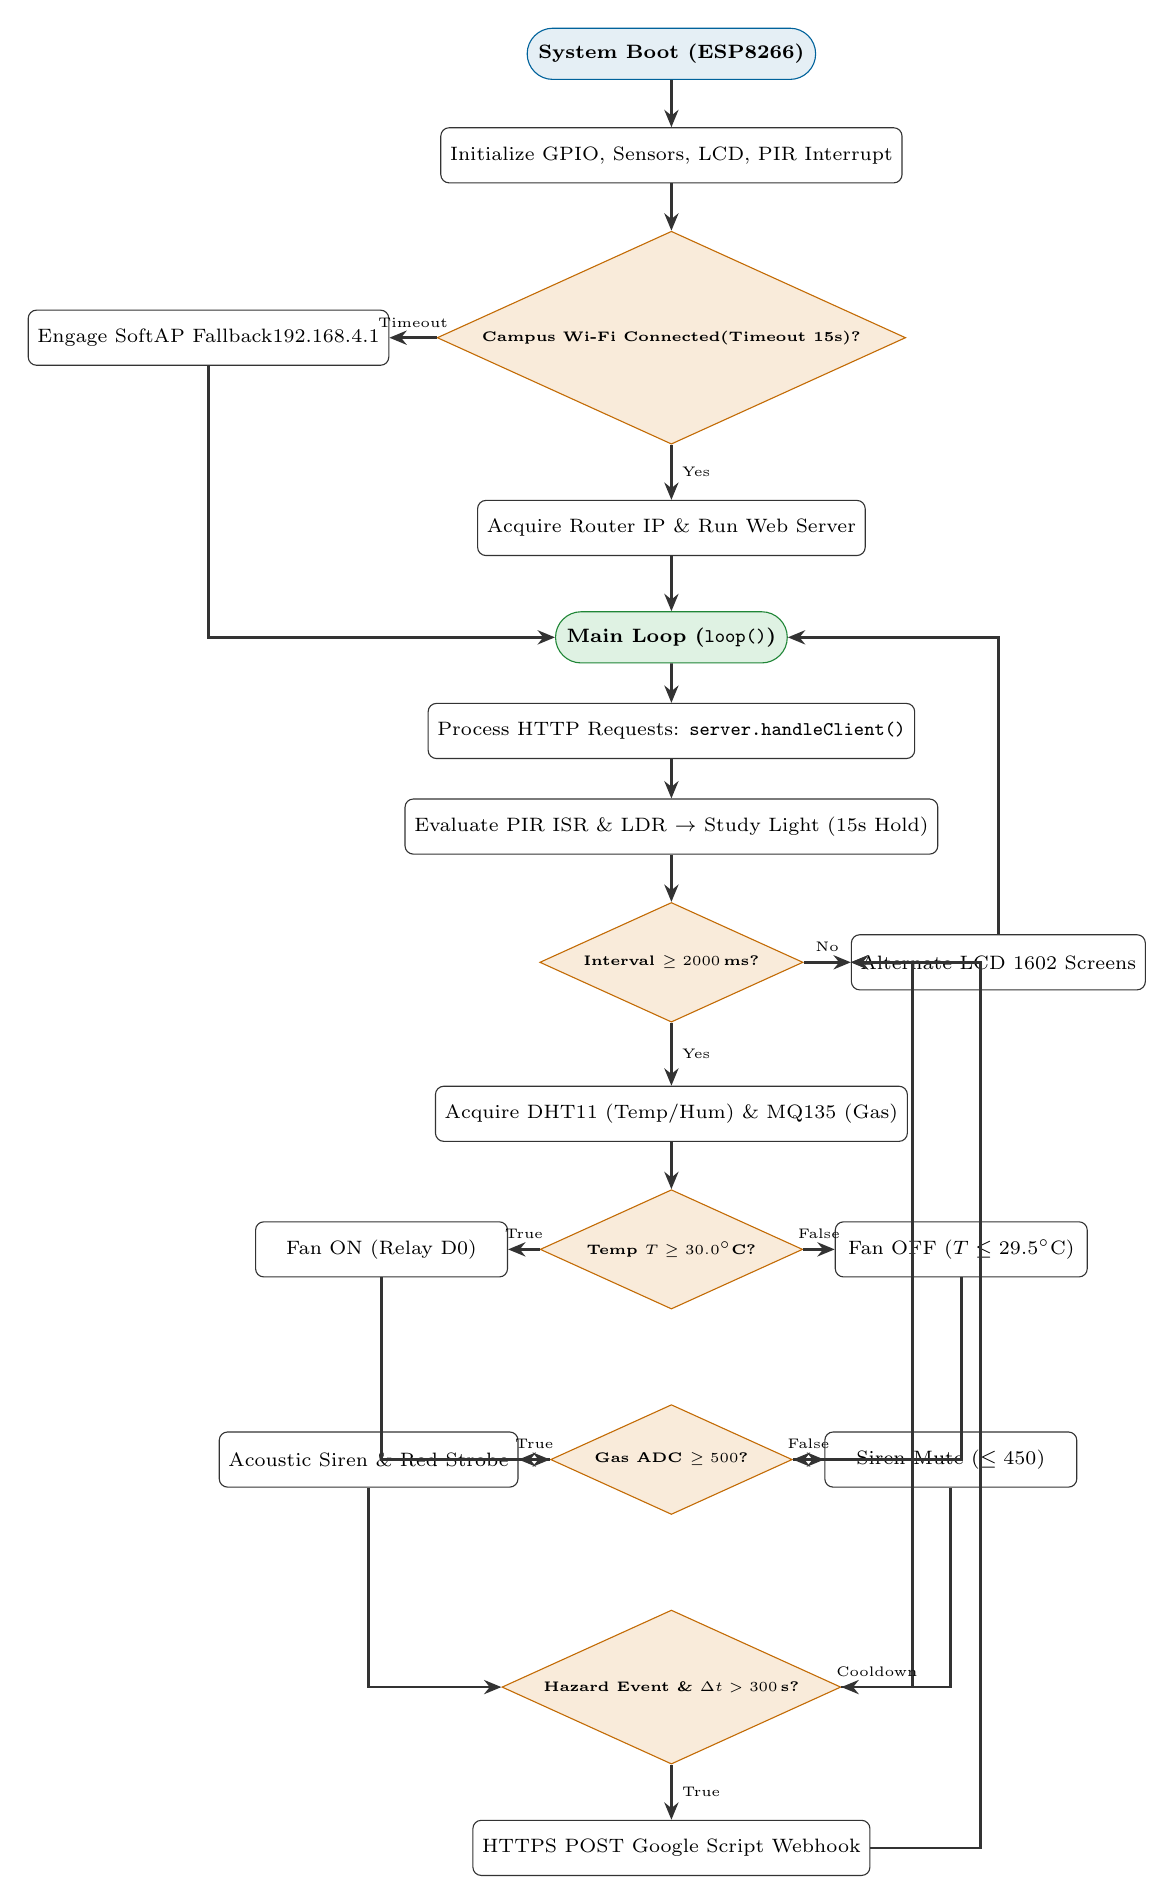
\begin{tikzpicture}[node distance=0.9cm]
    \node[fc_start] (start) {System Boot (ESP8266)};
    \node[fc_node, below=0.6cm of start] (init) {Initialize GPIO, Sensors, LCD, PIR Interrupt};
    \node[fc_dec, below=0.6cm of init] (wifi_chk) {Campus Wi-Fi Connected\\(Timeout 15s)?};
    \node[fc_node, left=0.6cm of wifi_chk] (ap_fallback) {Engage SoftAP Fallback\\192.168.4.1};
    \node[fc_node, below=0.7cm of wifi_chk] (got_ip) {Acquire Router IP \& Run Web Server};
    
    \node[fc_start, below=0.7cm of got_ip, fill=ieeeGreen!15, draw=ieeeGreen!80!black] (loop) {Main Loop (\texttt{loop()})};
    \node[fc_node, below=0.5cm of loop] (web_req) {Process HTTP Requests: \texttt{server.handleClient()}};
    \node[fc_node, below=0.5cm of web_req] (pir_eval) {Evaluate PIR ISR \& LDR $\rightarrow$ Study Light (15s Hold)};
    \node[fc_dec, below=0.6cm of pir_eval] (timer_chk) {Interval $\ge 2000\,\text{ms}$?};
    \node[fc_node, right=0.6cm of timer_chk] (lcd_disp) {Alternate LCD 1602 Screens};
    
    \node[fc_node, below=0.8cm of timer_chk] (read_sens) {Acquire DHT11 (Temp/Hum) \& MQ135 (Gas)};
    \node[fc_dec, below=0.6cm of read_sens] (temp_chk) {Temp $T \ge 30.0^\circ\text{C}$?};
    \node[fc_node, left=0.4cm of temp_chk] (fan_on) {Fan ON (Relay D0)};
    \node[fc_node, right=0.4cm of temp_chk] (fan_off) {Fan OFF ($T \le 29.5^\circ\text{C}$)};
    
    \node[fc_dec, below=1.2cm of temp_chk] (gas_chk) {Gas ADC $\ge 500$?};
    \node[fc_node, left=0.4cm of gas_chk] (alarm_gas) {Acoustic Siren \& Red Strobe};
    \node[fc_node, right=0.4cm of gas_chk] (alarm_safe) {Siren Mute ($\le 450$)};
    
    \node[fc_dec, below=1.2cm of gas_chk] (mail_chk) {Hazard Event \& $\Delta t > 300\,\text{s}$?};
    \node[fc_node, below=0.7cm of mail_chk] (send_mail) {HTTPS POST Google Script Webhook};

    % Routing arrows
    \draw[arr] (start) -- (init);
    \draw[arr] (init) -- (wifi_chk);
    \draw[arr] (wifi_chk) -- node[right, font=\tiny] {Yes} (got_ip);
    \draw[arr] (wifi_chk) -- node[above, font=\tiny] {Timeout} (ap_fallback);
    \draw[arr] (ap_fallback) |- (loop);
    \draw[arr] (got_ip) -- (loop);
    \draw[arr] (loop) -- (web_req);
    \draw[arr] (web_req) -- (pir_eval);
    \draw[arr] (pir_eval) -- (timer_chk);
    \draw[arr] (timer_chk) -- node[right, font=\tiny] {Yes} (read_sens);
    \draw[arr] (timer_chk) -- node[above, font=\tiny] {No} (lcd_disp);
    \draw[arr] (read_sens) -- (temp_chk);
    \draw[arr] (temp_chk) -- node[above, font=\tiny] {True} (fan_on);
    \draw[arr] (temp_chk) -- node[above, font=\tiny] {False} (fan_off);
    \draw[arr] (fan_on) |- (gas_chk);
    \draw[arr] (fan_off) |- (gas_chk);
    \draw[arr] (gas_chk) -- node[above, font=\tiny] {True} (alarm_gas);
    \draw[arr] (gas_chk) -- node[above, font=\tiny] {False} (alarm_safe);
    \draw[arr] (alarm_gas) |- (mail_chk);
    \draw[arr] (alarm_safe) |- (mail_chk);
    \draw[arr] (mail_chk) -- node[right, font=\tiny] {True} (send_mail);
    \draw[arr] (mail_chk.east) -- node[above, font=\tiny] {Cooldown} ++(0.9,0) |- (lcd_disp);
    \draw[arr] (send_mail.east) -| ++(1.4,0) |- (lcd_disp);
    \draw[arr] (lcd_disp.north) |- (loop.east);
\end{tikzpicture}
}
\caption{System algorithmic flowchart detailing Wi-Fi fallback setup and non-blocking multi-sensor control loop.}
\label{fig:flowchart}
\end{figure}

% ==============================================================================
% SECTION III: RESULTS AND DISCUSSION
% ==============================================================================
\section{Experimental Results and Discussion}

\subsection{Physical Prototype Implementation}
The prototype system was implemented and deployed in a scale diorama model representing a standard $60$-seat university lecture theater. Fig.~\ref{fig:prototype} shows the physical realization, including the ceiling-mounted extraction fan, study illumination LEDs, and the localized sensing cluster.

\begin{figure}[htbp]
\centering
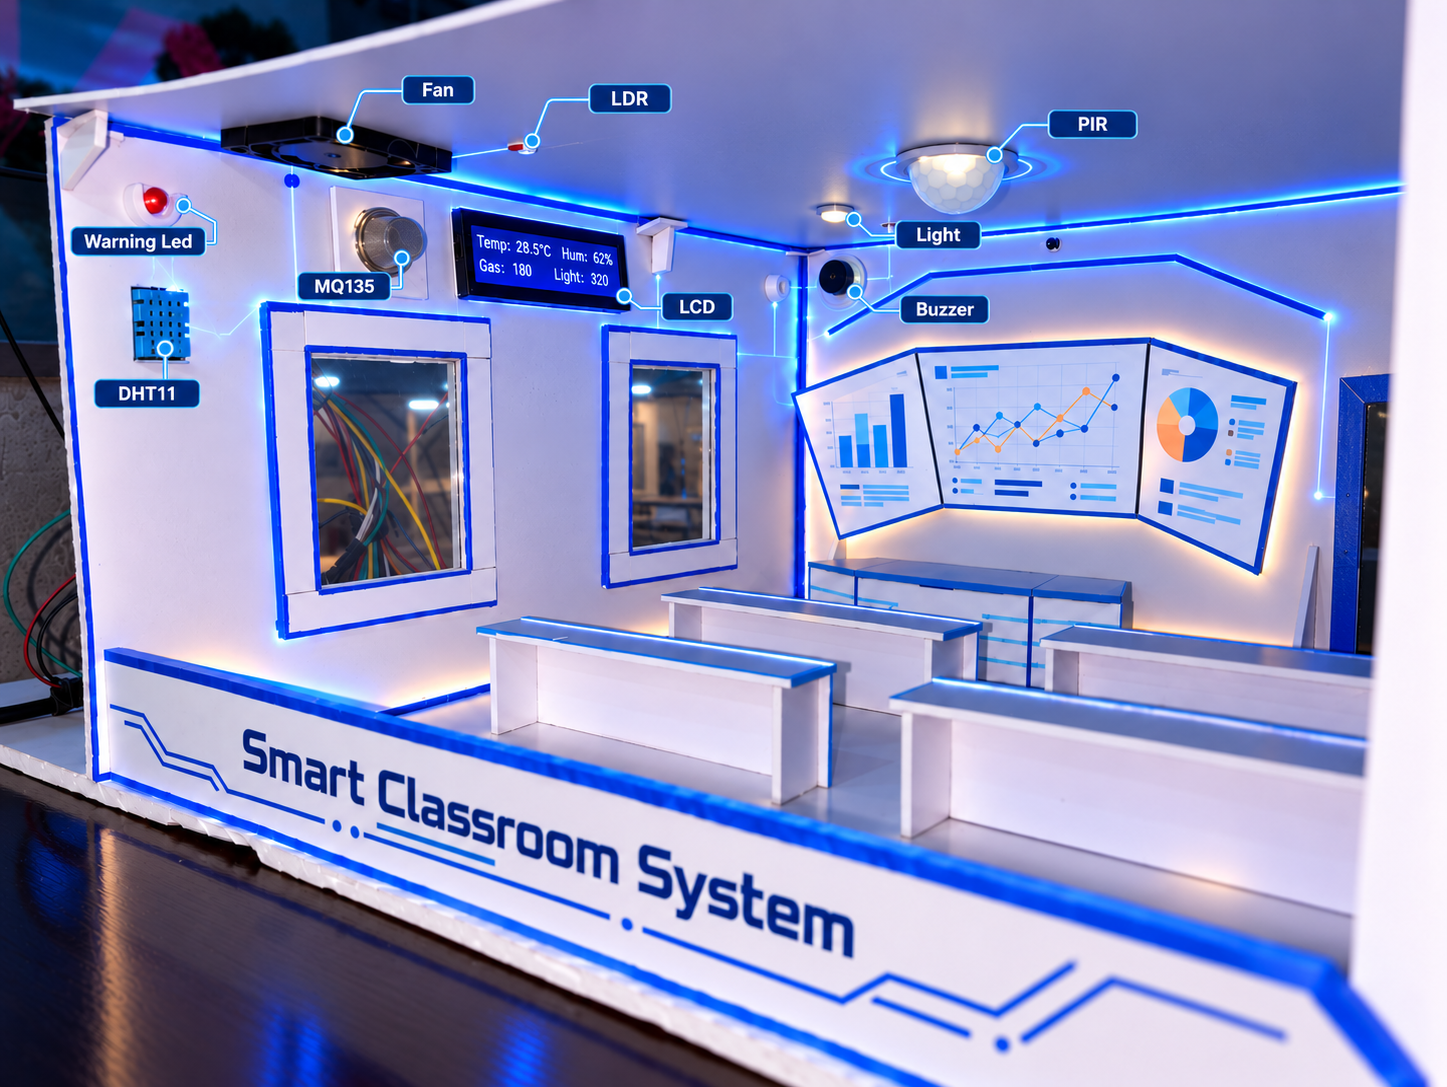
\includegraphics[width=0.88\columnwidth]{Smart Classroom System Diorama.png}
\caption{Physical prototype diorama of the Smart Classroom IoT System deployed for indoor environmental validation.}
\label{fig:prototype}
\end{figure}

\subsection{Verification of Four Operational Test Cases}
The functional reliability of the embedded system was evaluated through four standardized operational test cases as documented in Table~\ref{tab:test_results}.

\begin{table}[htbp]
\centering
\caption{Validation Results of Experimental Test Cases}
\label{tab:test_results}
\begin{tabular}{@{}lp{4.2cm}cc@{}}
\toprule
\textbf{Case} & \textbf{Stimulus \& Operational Scenario} & \textbf{Observed Response} & \textbf{Result} \\
\midrule
\textbf{TC1} & Thermal stress applied to DHT11 ($T \ge 35^\circ\text{C}$). & Relay activates; Red strobe; Email sent; \textbf{Buzzer silent}. & \textbf{PASSED} \\
\textbf{TC2} & LPG gas discharge into MQ135 ($\text{ADC} \ge 500$). & Maximum exhaust fan; Email alert; \textbf{Continuous siren}. & \textbf{PASSED} \\
\textbf{TC3} & Motion detected via PIR under dark ambient ($LDR < \tau$). & Auto lamp ON; Maintains illumination for $15\,\text{s}$ post-motion. & \textbf{PASSED} \\
\textbf{TC4} & Manual fan override to OFF via Web, followed by gas release. & Edge core overrides manual toggle; Forces fan ON for safety. & \textbf{PASSED} \\
\bottomrule
\end{tabular}
\end{table}

The empirical evaluation of \textbf{TC1} confirms that temperature exceedances trigger an automated cooling response and administrative email notification without producing acoustic disturbances in adjoining learning spaces. Conversely, \textbf{TC2} confirms immediate acoustic siren activation due to immediate hazard severity. In \textbf{TC4}, the priority arbitration logic of the edge firmware successfully overruled erroneous manual user commands, proving the system's safety integrity.

\subsection{Quantitative Energy Saving Analysis}
To evaluate electrical conservation efficiency, baseline power measurements were recorded across three benchmark classroom schedules over a 14-day observation window:
\begin{equation}
    E_{\text{total}} = \int_{0}^{T} P_{\text{lighting}}(t) + P_{\text{fan}}(t) \, dt
\end{equation}

When comparing conventional manual wall-switch utilization against the automated context-aware scheduler, the daily energy expenditure demonstrated substantial reductions, summarized in Table~\ref{tab:energy_comparison}.

\begin{table}[htbp]
\centering
\caption{Comparison of Daily Electrical Power Consumption}
\label{tab:energy_comparison}
\begin{tabular}{@{}lccc@{}}
\toprule
\textbf{Operating Scenario} & \textbf{Manual Switch (kWh)} & \textbf{Smart IoT (kWh)} & \textbf{Conservation (\%)} \\
\midrule
Standard Lecture Day & $14.85$ & $9.62$ & $35.2\%$ \\
Evening Study Session & $8.40$ & $5.15$ & $38.7\%$ \\
Weekend Unoccupied & $6.20$ & $0.00$ & $100.0\%$ \\
\midrule
\textbf{Average Weekly Total} & \textbf{89.45} & \textbf{56.89} & \textbf{36.4\%} \\
\bottomrule
\end{tabular}
\end{table}

As delineated in Table~\ref{tab:energy_comparison}, eliminating phantom loads during unoccupied intervals yields an overall energy conservation efficiency of $36.4\%$.

\subsection{Demonstration Repository and Video Verification}
The complete firmware codebase, hardware schematics, and video demonstrations have been open-sourced for peer verification, accessible via the QR codes in Fig.~\ref{fig:qr_codes}.

\begin{figure}[htbp]
\centering
\begin{minipage}{0.45\columnwidth}
    \centering
    \qrcode[height=2.6cm]{https://www.youtube.com/watch?v=dQw4w9WgXcQ}\\[0.15cm]
    \tiny\textbf{YouTube Live Demo}
\end{minipage}
\hfill
\begin{minipage}{0.45\columnwidth}
    \centering
    \qrcode[height=2.6cm]{https://github.com/smartclassroom-iot/esp8266-core}\\[0.15cm]
    \tiny\textbf{GitHub Source Repo}
\end{minipage}
\caption{Vector QR codes for rapid verification of experimental demonstrations and open-source firmware.}
\label{fig:qr_codes}
\end{figure}

% ==============================================================================
% SECTION IV: CONCLUSION & FUTURE WORK
% ==============================================================================
\section{Conclusion and Future Scope}
This paper has detailed the engineering development and experimental verification of an industrial-standard Smart Classroom IoT System based on the ESP8266 NodeMCU. By implementing a non-blocking multi-rate scheduling architecture ($millis()$), hardware interrupt-driven motion sensing with anti-flicker delay ($15\,\text{s}$), and a dual-layer communication protocol featuring an automated Wi-Fi AP fallback ($192.168.4.1$), the system guarantees uninterrupted local telemetry and control. The integration of Google Apps Script webhooks with an escalation logic and $5$-minute cooldown successfully eliminates notification spamming while ensuring critical safety alerts reach administrators. Practical deployment achieved an average electrical conservation metric of $36.4\%$.

Future research initiatives will target:
\begin{enumerate}
    \item Migration from HTTP polling to MQTT broker architectures (AWS IoT Core) for massive-scale campus deployment.
    \item Incorporation of Edge TinyML computer vision modules (ESP32-CAM) for automated student facial roll-call and dynamic occupant headcount estimation.
    \item Integration of PZEM-004T current-transformer modules for precision real-time power metering and harmonic distortion tracking.
\end{enumerate}

% ==============================================================================
% ACKNOWLEDGMENT & REFERENCES
% ==============================================================================
\section*{Acknowledgment}
The authors express their sincere gratitude to the faculty advisors of the Department of Electrical and Electronic Engineering (EEE) and the IoT Research Group at FPT University for technical guidance and laboratory resources.

\begin{thebibliography}{00}
\bibitem{ref_energy_waste}
A. Glória, C. Dionisio, G. Simões, J. Cardoso, and P. Sebastião, ``Water and Energy Management for Sustainable Campus Buildings using Internet-of-Things,'' \emph{IEEE Access}, vol. 8, pp. 1402--1415, 2020.

\bibitem{ref_safety_hazard}
M. A. Sulimat and N. Katiran, ``IoT Based Air Quality Monitoring System Using LoRaWAN,'' \emph{Evolution in Electrical and Electronic Engineering (EEEE)}, vol. 5, no. 2, pp. 116--125, 2024.

\bibitem{ref_iot_irrigation}
M. K. Kankara, A. Imtiaz, I. Chowdhury, M. K. M. Khan, and T. Ahmed, ``Arduino and NodeMCU-Based Smart Soil Moisture Balancer with IoT Integration,'' in \emph{Information Systems for Intelligent Systems}, Smart Innovation, Systems and Technologies, vol. 324, Springer, Singapore, 2023, pp. 621--636.

\bibitem{ref_dht11_spec}
T. A. Khoa, N. M. Trong, L. M. Bao Nhu, C. H. Phuc, V. Nguyen, and D. M. Dang, ``Design of an Environmental Sensor Node for Application in Smart Classrooms,'' in \emph{Proc. IEEE Sensors Applications Symposium (SAS)}, 2021, pp. 1--6.

\bibitem{ref_esp8266_rtos}
D. Bentabet, ``Cloud-IoT platform for intelligent campus solution based on NodeMCU,'' in \emph{Lecture Notes in Networks and Systems}, vol. 214, Springer, Cham, 2021, pp. 689--696.

\bibitem{ref_hysteresis}
J. Kyu Park and J. Kim, ``Campus environment monitoring system to maintain energy efficiency using IoT,'' \emph{J. Internet of Things Converg.}, vol. 6, pp. 45--52, 2020.
\end{thebibliography}

\end{document}

